% This percent indicates a comment.
% This is a very simple latex article that introduces the way 
% equations are typeset.  Do this in linux:
%
% latex first.tex
% latex first.tex
% xdvi first.dvi
% dvips -o first.ps first.dvi
% gv first.ps
% lpr first.ps
% pdflatex first.tex
% acroread first.pdf
\documentclass[11pt,a4paper]{article}
\usepackage[utf8]{inputenc}
\usepackage[english]{babel}
\usepackage[T1]{fontenc}
\usepackage{graphicx}
\usepackage{verbatim}
\usepackage{url}
\usepackage{fancyhdr}
\pagestyle{fancy}
\title{Identification and Archiving of the Czech~Web Outside the National Domain}
\author{Ivan Vlček}
\date{05.06.2008}

\begin{document}

\begin{center}
\thispagestyle{empty}

\huge{Identification and Archiving of the Czech Web Outside the National Domain}

\vspace{5em}

\large{Ivan Vlček}

\normalsize{6 May, 2008}

\newpage
\thispagestyle{empty}
\tableofcontents

\end{center}
\newpage

%================================NEW SECTION================================%

\section{Introduction}

The placement of different documents on the Internet has recently become very popular. Internet users find this feature helpfull, because new documents can be uploaded on the Internet in relatively small effort. Some of these documents are considered to be very important in spheres such as hi\-sto\-ry, science, art and so forth. But there exists a risk that the information will be changed, or even deleted and lost forever. Therefore it's our duty to save this sort of documents for future generation.

The question of archiving the Internet content is solved by many institutions. The most famous is called Internet Archive that creates Internet library and provides access to archival collection.

There is a project called WebArchiv in Czech Republic that manages archiving of Czech web and ensures access to archival collection. The only criterion how to identify the czech webpage operates on the basis of domain. This ensures all URLs with czech domain are archived. But there are also websites considered to be czech, whose domain is different from cz, e.g. .net, .com, .org, edu. The WebArchiv is interested in these websites and therefore one of the latest goal is archiving the Czech web outside the national domain.

This work describes the system to identify and archive the Cech web outside the national domain. The system for identifying the Czech web is called a WebAnalyzer and is integrated in an open-source software Heritrix, which is able to archive webpages. With this system it's possible to identify the Bohemian source on the basis of many criteria included in the system. The Bohemian source is every document that meets conditions specified by user. Having received confirmation from WebAnalyzer that the processed URI is identified as Bohemian URI, Heritrix archives it.

%================================NEW SECTION================================%

\newpage
\section{The WebArchiv Project}

Main task of the project WebArchiv is archiving and providing access to the archival collecton of Czech web. The WebArchiv uses web crawlers to perform comprehensive harvesting of national domain. Heritris seems to be suitable tool for this kind of work, because it's modular, extendible and everyone finds it easy to configure the crawl job. The Heritrix provides a lot of configurable modules that can be combined together and this gives you many creative possibilities to specify the crawl job you need. And if you demand some new functionality, it's possible to develop new module and attach it to Heritrix.

\subsection*{The Comprehensive Harvesting of Czech Web}
Heritrix performs the comprehensive harvesting on basis of modules, that filters out all URIs whose domain differs from .cz. All Czech webpages, that pass through the processors and deciding rules are archived. Discovered links with czech domain are further included into the collection of waiting URIs, while other links with different domains are ignored and marked as \emph{out of scope}.

\subsection*{The Comprehensive Harvesting of Czech Web Outside the National Domain}
Harvesting of Czech web outside the national domain should follow the harvesting of Czech web. 

The \emph{out of scope} links, that comes out from harvesting of Czech web are valuable input material for following harvesting of Czech web outside the national domain. There is a chance that these links reffered from czech webpages lead to Bohemian sites. Therefore it's convenient to start crawling with these URIs. The \emph{out of scope} links will represent seeds for new crawl job of harvesting outside the national domain.

%================================NEW SECTION================================%

\newpage
\section{Heritrix}

Heritrix is able to do both, crawl web and archive it. It's open-source software written in Java, that provides user-friendly web interface. User manual is available on \url{http://crawler.archive.org}. Before describing the WebAnalyzer, we should know how Heritrix works.

\subsection{A brief Overview}
Heritrix is designed to be modular. Which modules to use can be set at runtime from the user interface. If you demand new functionality, you can implement new module and attach it to Heritrix, or you can replace existing module.

The crawler consists of core classes and pluggable modules. The core classes can be configured, but not replaced. The pluggable classes can be substituted by altering the configuration of the crawler. A set of basic pluggable classes are shipped with the crawler, but if you have needs not met by these classes you could write your own.

\begin{center}
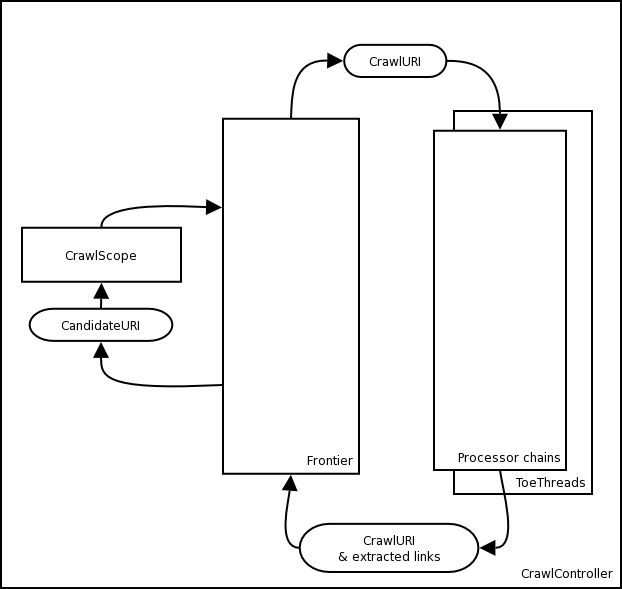
\includegraphics[width=120mm]{crawler_overview1.png}
\end{center}

\subsection{The CrawlController}
The CrawlController collects all the classes which cooperate to perform a crawl, provides a high-level interface to the running crawl, and executes the "master thread" which doles out URIs from the Frontier to the ToeThreads. As the "global context" for a crawl, subcomponents will usually reach each other through the CrawlController.

\subsection{The Frontier}
The Frontier is responsible for handing out the next URI to be crawled. It is responsible for maintaining politeness, that is making sure that no web server is crawled too heavily. After a URI is crawled, it is handed back to the Frontier along with any newly discovered URIs that the Frontier should schedule for crawling.

It is the Frontier which keeps the state of the crawl. This includes, but is not limited to:

\begin{itemize}
\item What URIs have been discovered
\item What URIs are being processed (fetched)
\item What URIs have been processed
\end{itemize}

The Frontier implements the Frontier interface and can be replaced by any Frontier that implements this interface. It should be noted though that writing a Frontier is not a trivial task.

The Frontier relies on the behavior of at least the following external processors: PreconditionEnforcer, LinksScoper and the FrontierScheduler (See below for more each of these Processors). The PreconditionEnforcer makes sure dns and robots are checked ahead of any fetching. LinksScoper tests if we are interested in a particular URL -- whether the URL is 'within the crawl scope' and if so, what our level of interest in the URL is, the priority with which it should be fetched. The FrontierScheduler adds ('schedules') URLs to the Frontier for crawling.

\subsection{ToeThreads}
The Heritrix web crawler is multi threaded. Every URI is handled by its own thread called a ToeThread. A ToeThread asks the Frontier for a new URI, sends it through all the processors and then asks for a new URI.

\subsection{Processors}
Processors are grouped into processor chains. Each chain does some processing on a URI. When a Processor is finished with a URI the ToeThread sends the URI to the next Processor until the URI has been processed by all the Processors. A processor has the option of telling the URI to skip to a particular chain. Also if a processor throws a fatal error, the processing skips to the Post-processing chain.

\begin{center}
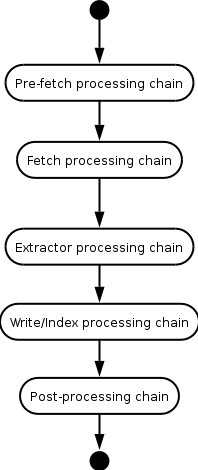
\includegraphics[width=40mm]{processing_steps.png}
\end{center}

The task performed by the different processing chains are as follows:

\subsubsection{Pre-fetch processing Chain}
The first chain is responsible for investigating if the URI could be crawled at this point. That includes checking if all preconditions are met (DNS-lookup, fetching robots.txt, authentication). It is also possible to completely block the crawling of URIs that have not passed through the scope check.

In the Pre-fetch processing chain the following processors should be included (or replacement modules that perform similar operations):

\begin{description}
\item[Preselector] Last check if the URI should indeed be crawled. Can for example recheck scope. Useful if scope rules have been changed after the crawl starts. The scope is usually checked by the LinksScoper, before new URIs are added to the Frontier to be crawled. If the user changes the scope limits, it will not affect already queued URIs. By rechecking the scope at this point, you make sure that only URIs that are within current scope are being crawled.
\item[PreconditionEnforcer] Ensures that all preconditions for crawling a URI have been met. These currently include verifying that DNS and \\robots.txt information has been fetched for the URI.
\end{description}

\subsubsection{Fetch processing Chain}
The processors in this chain are responsible for getting the data from the remote server. There should be one processor for each protocol that Heritrix supports: e.g. FetchHTTP.

\subsubsection{Extractor processing Chain}
At this point the content of the document referenced by the URI is available and several processors will in turn try to get new links from it.

\subsubsection{Write/Index processing Chain}
This chain is responsible for writing the data to archive files. Heritrix comes with an ARCWriterProcessor which writes to the ARC format. New processors could be written to support other formats and even create indexes.

\subsubsection{Post-processing Chain}
A URI should always pass through this chain even if a decision not to crawl the URI was done in a processor earlier in the chain. The post-processing chain must contain the following processors (or replacement modules that perform similar operations):

\begin{description}
\item[CrawlStateUpdater] Updates the per-host information that may have been affected by the fetch. This is currently robots and IP address info.
\item[LinksScoper] Checks all links extracted from the current download against the crawl scope. Those that are out of scope are discarded. Logging of discarded URLs can be enabled.
\item[FrontierScheduler] 'Schedules' any URLs stored as CandidateURIs found in the current CrawlURI with the frontier for crawling. Also schedules prerequisites if any.
\end{description}

Further information are available in developer manual \url{http://crawler.archive.org/articles/developer_manual/index.html}.

%================================NEW SECTION================================%

\newpage
\section{The Integration}

It's very important to integrate the WebAnalyzer into the Heritrix properly for us to reach required behaviour. The WebAnalyzer must analyze every URI, that goes through the process of crawling. Therefore it's necessary to integrate the WebAnalyzer into some module that will be used by Heritrix.

A good idea is to implement the WebAnalyzer as a standalone module with defined inteface, that will be used by some module in Heritrix. The simple input for WebAnalyzer should be the URI, about which it decides whether it is the Bohemian URI or not. The output for Heritrix should be the logical value (\emph{true} if analyzed URI is marked as Bohemian URI and \emph{false} otherwise). The next important thing, is to choose the proper Heritrix module, into which we integrate the WebAnalyzer.

The WebAnalyzer should start analyzing the URI, after Heritrix gets the biggest possible amount of information about processed URI.

% integration into Frontier
Integration into Frontier is not possible due to two reasons. The Frontier has access to processed URI at the very beginning or at the very end of crawling. At the beginning there are almost no discovered information about URI. At the end of processing Heritrix discovered much information about URI, but at this point it's not possible to archive Bohemian URI. Archiving is executed by ARCWriterProcessor that is performed before URI finishes in Frontier. Both of these possibilities aren't convenient. We have to integrate the WebAnalyzer into module, that will be executed before \mbox{ARCWriterProcessor}, so that we can decide whether the processed URI has to be archived.

% integration into Filter
Integration into module Filter seemed to be conveniet, because Filter can be placed at any point in the process of crawling. Configurable Filter checks whether processed URL meets all specified criteria. It would be pretty easy to place the Filter before ARCWriterProcessor and use the WebAnalyzer in Filter to identify the URI. Having tried this possibility, we noticed the problem with initialization of WebAnalyzer. Before analyzing the processed URI, the WebAnalyzer has to be initialized, so that the database connections used by WebAnalyzer can be established. The Filter's interface doesn't provide suitable interface for this job.

% integration into Scope
Integration into module Scope meets requirements for initializing and closing the WebAnalyzer instance. But the Interne Archive posted, that the Scope module would be completely reorganized in the next version of Heritrix, so we better tried another possible way.

% integration into Processor
Integration into module Processor was the final and right possibility. While testing the first version with processor, we found out that the integration in processor is the most suitable way. Processors are grouped in processor chains as we described above. We chose the extractor processing chain for the WebAnalyzer, because at this point the content of the document referenced by the URI is available and several processors such as ExtractorHTML and ExtractorCSS discovered new links from it. Therefore we have to implement new Extractor, that will be placed at the end of extractor processing chain, when all information (content type, text content, discovered links) will be available.

Next chain is write/index processing chain that archives URI and last chain is called post-processing chain, that filters out discovered links according to definition specified by user. Having been processed by post-processing chain, the URI finishes in Frontier again. After all discovered links on this URI are scheduled in Frontier, the process of crawling the URI ends.

The Extractor provides \emph{initialize()} and \emph{finalize()} methods. All Processors are initialized by \emph{initialize()} method at the beginning of the crawl job and at the end \emph{finalize()} method is called by CrawlController to finalze all used Processors. We can simply use these methods to initialize and close WebAnalyzer instance. In the main method of Extractor, called \emph{innerProcess(CrawlURI\footnote{CrawlURI is URI object that is just processed by processors and is associated with one ToeThread} curi)}, we can use the WebAnalyzer to identify the processed CrawlURI. Only CrawlURI identified as Bohemian URI is archived by ARCWriterProcessor.

After implementing and testing the first version with Extractor module, we noticed several imperfections. The system wasn't able to archive images, css styles, links and other sources placed on the Bohemian URI. The integration must be done by more modules, to solve these problems.

\subsection{The Integration by Modules}
On the basis of new requirements the use case diagram was created, to describe the intregration of WebAnalyzer into Heritrix. The integration is realized by modules ExtractorWebAnalyzer, ARCWriterProcessorWebAnalyzer and LinksScoperWebAnalyzer. The ExtractorWebAnalyzer is the only one, that directly uses the interface of WebAnalyzer module.

\begin{center}
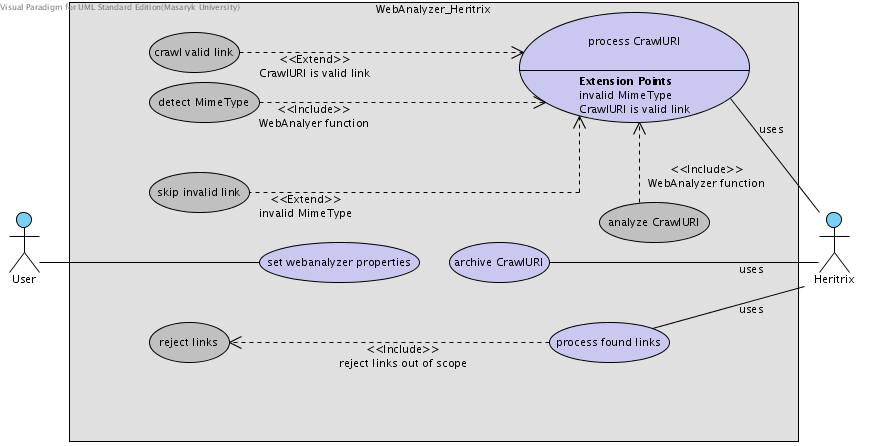
\includegraphics[width=130mm]{usecase1.png}
\end{center}

\subsubsection{The Archiving of DNS Records}
Before processing any webpage, Heritrix automaticaly archives all asso\-cia\-ted DNS records. We don't need all these DNS records but only those of Bohemian URI. It's hard to reach this state, therefore we use our own ARCWriterProcessorWebAnalyzer, that simply ignores all DNS records so far.

\subsubsection{The Mime Type Detector}
While testing the first version, we noticed many \emph{java.lang.OutOfMemory} exceptions caused by analyzing the documents, the Mime type of which was wrong detected by Heritrix.

Old servers unable to identify the type of document, set \emph{text/plain} value as content type for each document. The WebAnalyzer analyzed only documents of text type, but actually they could be audio or video documents, the size of which can take hundreds of MB. The text analyzing led to creating huge \emph{java.lang.String} objects, that caused \emph{java.lang.OutOfMemory} exceptions. The functionality of Heritrix to identify the content type of document is not sufficient and therefore we have to implement some sort of Mime Type detector, that will identify the content type of document before it will be analyzed by WebAnalyzer. This ensures that documents of binary content won't be analyzed by WebAnalyzer.

\subsubsection{The Archiving of Links and Images}
\label{aolai}
The first version archives only Bohemian URI. Other URIs (images, css, other multimedia sources) associated with this Bohemian URI are not archived. But we need to archive not only sources associated with Bohemian URI but also its links. Links referenced from Bohemian URI can carry worth information and it's good idea to archive them to defined depth from Bohemian URI.

\begin{center}
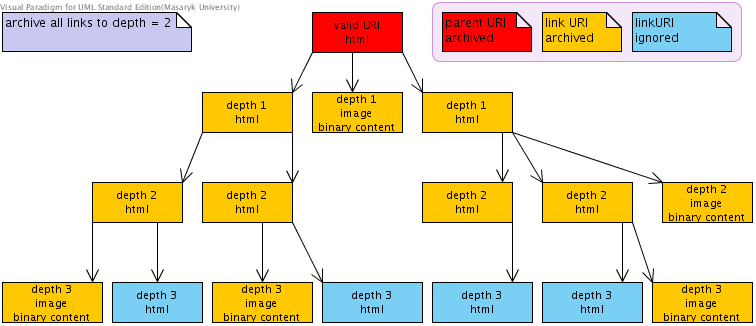
\includegraphics[width=120mm]{depth.png}
\end{center}

Picture shows a tree with Bohemian URI as root. The nodes are links referenced from Bohemian URI (images, css styles, other html pages). If the defined depth equals 2, than all links have to be archived to this level (see picture). But if the document on the second level is html page, than it will be archived without its images, css styles and other sources. Therefore we have to archive all documents from the third level except of html documents. This ensures that all images and other sources placed on archived html page will be achived as well. User is able to define the depth's value before starting the crawl job of Heritrix.

Realization of archiving links and images required new module Links\-ScoperWebAnalyzer and some changes in ExtractorWebAnalyzer, so that these modules could cooperate together. Objects CrawlURI and CandidateURI\footnote{CandidateURI represents URI referenced from CrawlURI. When CandidateURI is going to be crawled, it turns to CrawlURI object.} are able to remember any information during the process of their crawling. And this is the way how we force the Heritrix to maintain the state of archiving the links and images. Module LinksScoperWebAnalyzer extends original module LinksScoper, but adds the functionality to handle links referenced from Bohemian URI.

Lets describe the workflow of archiving links from Bohemian URI:

\begin{center}
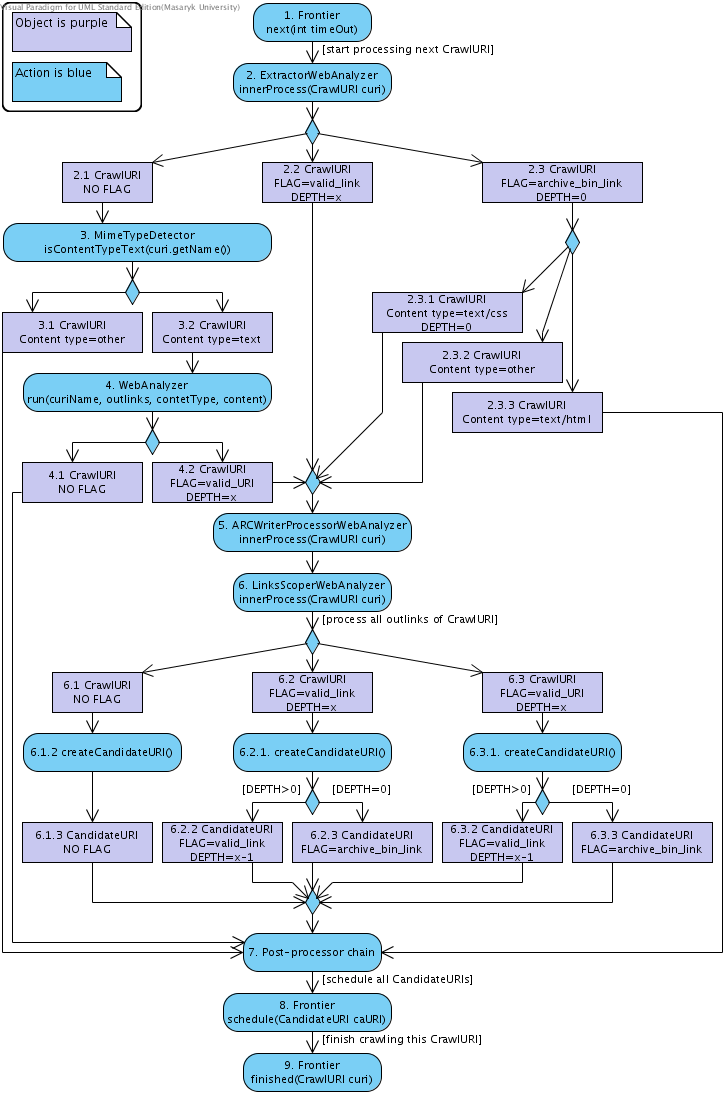
\includegraphics[width=120mm]{archiveLinks.png}
\end{center}

\begin{description}
\item[1. Frontier next(int timeout)] - Having been called by ToeThread, the CrawlURI entered the process of crawling. Each URI is stored and scheduled in Frontier object and waits for ToeThread to be crawled. While crawling, the CrawlURI is processed by processors defined by user.
\item[2. ExtractorWebAnalyzer innerProcess(CrawlURI curi)] - After the CrawlURI reaches the ExtractorWebAnalyzer, it is checked whether it contains some flag. Next processing depedns on the flag's value.

\begin{description}
\item[2.1 CrawlURI NO FLAG] - The CrawlURI has no flag. WebAnalyzer will identifiy its mime type with MimeTypeDetector.
\item[2.2 CrawlURI FLAG=valid\_link, DEPTH=x] - The CrawlURI has the flag \emph{valid\_link} determining that this CrawlURI was re\-fe\-ren\-ced from Bohemian URI and it has to be archived immediately. WebAnalyzer doesn't analyze this CrawlURI, it would do it in vain. The CrawlURI is sent directly to ARCWriterProcessorWebAnalyzer to be archived. The \emph{DEPTH=x} determines the level, to which the links discovered on this CrawlURI has to be archived as well.
\item[2.3 CrawlURI FLAG=archive\_bin\_link, DEPTH=0] - The \\CrawlURI with this flag determines, that this URI is referenced from Bohemian URI. We have to archive all CrawlURIs with this flag except of html pages to ensure that all images and other sources referenced from Bohemian URI will be archived. Crawl\-URI\-s with this flag represent the lists of tree. See picture \S\ref{aolai}.

\begin{description}
\item[2.3.1 CrawlURI Content type=text/css, DEPTH=0] - If \\the CrawlURI with flag \emph{archive\_bin\_link} is a document of type \emph{text/css}, we have to archive it immediately and also set new flag \emph{valid\_link, DEPTH=0} for this CrawlURI. This ensures that all links referenced from css document will be archived. 
\item[2.3.2 CrawlURI Content type=other] - CrawlURI with flag \emph{archive\_bin\_link}, the content type of which differs from \\ \emph{text/html}, has to be archived. This ensures all multimedia sources from Bohemian URI will be in archival collection.
\item[2.3.3 CrawlURI Content type=text/html] - CrawlURI with \emph{archive\_bin\_link} flag, the content type of which is \emph{text/html} will not be archived. This ensures that the depth defined by user will not be exceeded.
\end{description}
\end{description}


\item[3. MimeTypeDetector isContentTypeText(curi.getName())] - The \\CrawlURI with no flag is identified by MimeTypeDetector. According to the identified mime type, the next step is chosen.

\begin{description}
\item[3.1 CrawlURI Content type=other] - The CrawlURI which identified mime type is different from \emph{text} will not be analyzed. Pro\-bab\-ly it is a URI with binary content. This CrawlURI skips to post-processing chain.
\item[3.2 CrawlURI Content type=text] - The CrawlURI with \emph{text} content type will be analyzed by WebAnalyzer in next step.
\end{description}

\item[4. WebAnalyzer run(curiName, outlinks, contentType, content)] - \\All CrawlURIs in this branch are analyzed by WebAnalyzer. On the basis of CrawlURI's details, WebAnalyzer decides whether the CrawlURI is Bohemian URI or not.

\begin{description}
\item[4.1 CrawlURI NO FLAG] - CrawlURI is not identified as Bohemian URI. It skips to post-processing chain.
\item[4.2 CrawlURI FLAG=valid\_URI, DEPTH=x] - The CrawlURI is identified as Bohemian URI. The flag and depth attribute are associated with this CrawlURI.
\end{description}

\item[5. ARCWriterProcessorWebAnalyzer innerProcess(CrawlURI curi)] - This processor archives all CrawlURIs except of DNS records.
\item[6. LinksScoperWebAnalyzer innerProcess(CrawlURI curi)] - This \\processor handles all links discovered on CrawlURI. New CandidateURIs are created from discovered links and corresponding flags are associated with CandidateURIs.

\begin{description}
\item[6.1 CrawlURI NO FLAG] - The CrawlURI with no flag is processed in usual way.

\begin{description}
\item[6.1.2 createCandidateURI()] - The CandidateURI object is created from link.
\item[6.1.3 CandidateURI NO FLAG] - The CandidateURI whose parent CrawlURI doesn't contain any flag, has no flag as well.
\end{description}

\item[6.2 CrawlURI FLAG=valid\_link, DEPTH=x] - The CrawlURI with this flag is next processed according to the value of \emph{DEPTH} attribute.

\begin{description}
\item[6.2.1 createCandidateURI()] - The CandidateURI object is created from link.
\item[6.2.2 CandidateURI FLAG=valid\_link, DEPTH=x-1] - \\The CrawlURI with depth value \emph{x>0}. Flag \emph{valid\_link, \\DEPTH=x-1}, is set for newly created CandidateURI. When the depth value is \emph{x=0}, then the \emph{archive\_bin\_link} is associated with CandidateURI. This ensures that valid links from Bohemian URI will be archived until they reach the defined depth.
\item[6.2.3 CandidateURI FLAG=archive\_bin\_link] - The \\CrawlURI with depth value \emph{x=0}. The flag \emph{archive\_bin\_link} is associated with CandidateURI. This flag ensures, that all sources (images, css, ...) placed on the archived URI will be archived as well.
\end{description}


\item[6.3 CralURI FLAG=valid\_URI, DEPTH=x] - The CrawlURI \\with this flag is next processed according to the value of depth attribute.

\begin{description}
\item[6.3.1 createCandidateURI()] - The CandidateURI object is created from link.
\item[6.3.2 CandidateURI FLAG=valid\_link, DEPTH=x-1] - \\The CrawlURI with depth value \emph{x>0}. Flag \emph{valid\_link, \\DEPTH=x-1} will be associated with CandidateURI.
\item[6.3.3 CandidateURI FLAG=arhchive\_bin\_link] - The \\CrawlURI with depth value \emph{x=0}. Flag \emph{archive\_bin\_link} will be associated with CandidateURI.
\end{description}
\end{description}

\item[7. Post-processor chain] - Each CrawlURI must go through this processor chain.
\item[8. Frontier schedule(CandidateURI caURI)] - Schedules each CandidateURI to the collection of waiting URIs, according to the priority.
\item[9. Frontier finish(CrawlURI curi)] - After the CrawlURI is processed by all processors, the ToeThread calls finish method of Frontier object. This ToeThread is now free to process next URI.

\end{description}

%================================NEW SECTION================================%

\newpage
\section{WebAnalyzer}

The WebAnalyzer is realized as standalone module packaged into \emph{.jar} file. WebAnalyzer provides simple interface, that is used by ExtractorWebAnalyzer to identify the processed URI. WebAnalyzer identifies the processed URI on the basis of properties specified by user. These properties can be defined in external file \emph{webanalyzer.properies}. User is able to configure which componentes of WebAnalyzer he wants to use. Important thing is to specify conditions for valid URI.

WebAnalyzer is designed to be modular, so that new modules can be added. WebAnalyzer provides interfaces for new modules, so it is easy to implement new criterion(module) for identifying analyzed URI.

\subsection{Overview of Class Diagram}

WebAnalyzer consists of few packages.

\begin{center}
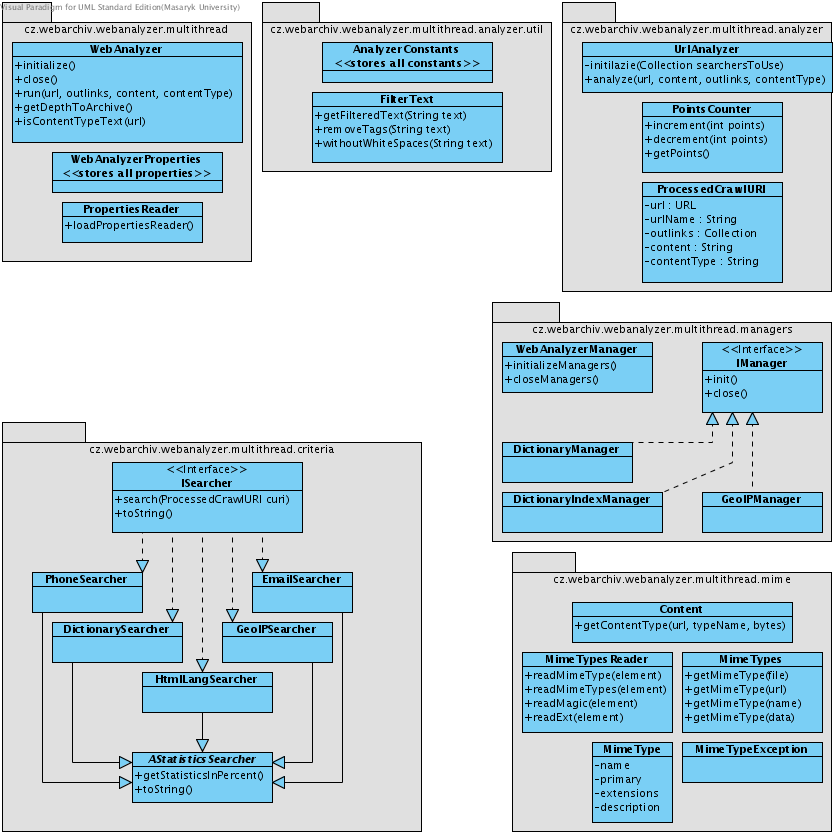
\includegraphics[width=120mm]{webanalyzerCD.png}
\end{center}

Lets describe the packages:

\begin{description}
\item[cz.webarchiv.webanalyzer.multithread] - This package contains classes that handles properties defined in \emph{webanalyzer.properties} file. There is also the main class that provides interface for using the WebAnalyzer.

\begin{description}
\item[WebAnalyzer] - This class provides interface for the whole system. This class is singleton (there is only one instance created during the process) and is directly used by ExtractorWebAnalyzer.
\item[PropertiesReader] - This class reads and validates the values of pro\-per\-ties defined in \emph{webanalyzer.properties} file.
\item[WebAnalyzerProperties] - This class stores the values for properties from \emph{webanalyzer.properties} file, for other objects to access these properties easily.
\end{description}

\item[cz.webarchiv.webanalyzer.multithread.analyzer.util] - This package \\contains classes with functions that are often used by the system.
\begin{description}
\item[FilterText] - This class provides functions for working with text.
\item[AnalyzerConstatns] - The class provides constants for better identification of criteria(modules) in source code.
\end{description}

\item[cz.webarchiv.webanalyzer.multithread.analyzer] - This package contains classes that stores the actual state of analyzing. All components cooperate with this package.
\begin{description}
\item[UrlAnalyzer] - The class that initializes all required criteria(com\-po\-nent\-s) and executes the analyzing. This class also counts statistics and decides whether the analyzed URI is valid or not.
\item[PointsCounter] - This class stores reached points for analyzed URI. If some component finds the relevant information, the PointsConter increments its points. At the end of analyzing reached points are compared with defined amount of points required for valid URI.
\item[ProcessedCrawlURI] - This class stores information about processed URI (name, content, content type, links).
\end{description}

\item[cz.webarchiv.webanalyzer.multithread.mime] - This package represents components that identify the mime type or URI.
\begin{description}
\item[Content] - This class provides interface to call the main method that identifies the mime type of URI. This class initializes all other objects needed for identifying.
\item[MimeType] - The class that stores information about mime type.
\item[MimeTypes] - This class stores all MimeType objects and is able to identify the mime type of unkonwn document on the basis of its(todo its) name or content.
\item[MimeTypesException] - The Exception that is thrown if some error occurs.
\end{description}

\item[cz.webarchiv.webanalyzer.multithread.managers] - This package contains classes that are neccessary for some searchers(components). I\-Ma\-na\-ger objects initializes database connections and opens necessary files.
\begin{description}
\item[WebAnalyzerManager] - The main class that initializes all objects of type IManager. At the end of the whole process this object closes all used managers.
\item[IManager] - IManager is interface, that all managers must implement. The Methods of managers that access to files and databases are usually synchronized, so that many threads can use the Web\-A\-na\-lyzer instance.
\end{description}

\item[cz.webarchiv.webanalyzer.multithread.criteria] - This package contains searchers. Each serchers represents some criterion. All searchers must implement ISeacher interface.
\begin{description}
\item[ISearcher] - The interface ISeacher requires \emph{search(ProcessedCrawlURI curi)} method and \emph{toString()} method. First method searches concrete information in object ProcessedCrawlURI and the other method provides statistics of analyzing.
\end{description}

\end{description}

%================================NEW SECTION================================%

\newpage
\section{Workflow}

Workflow of identifing the URI is divided into 4 parts. Each part represents one method, that is called from Heritrix.

\subsection{The Initialization}

\begin{center}
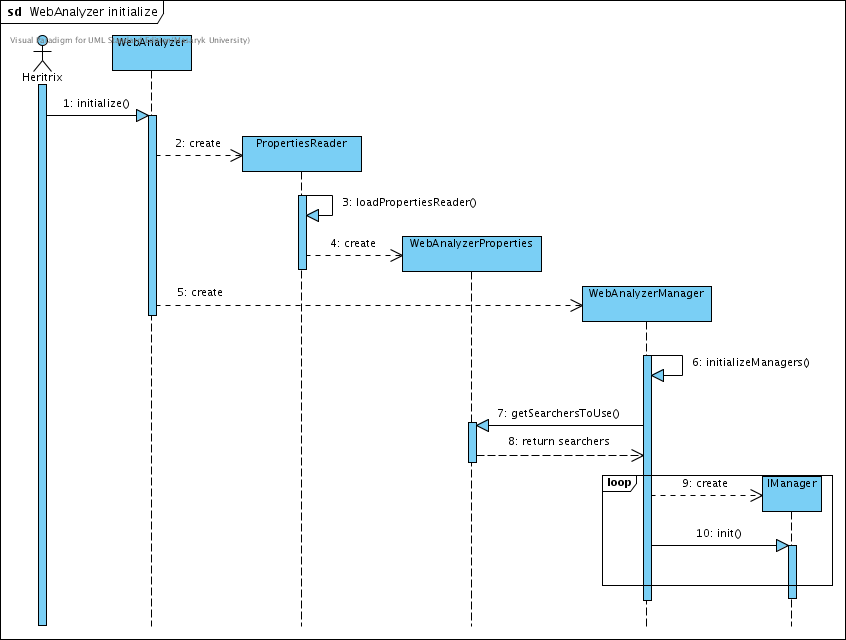
\includegraphics[width=120mm]{SD1.png}
\end{center}

Before using the WebAnalyzer, it's necessary to initialize it. The i\-ni\-tia\-li\-za\-tion is performed simultaneously with the initialization of Extractor\-Web\-Analyzer. There is only one instance of WebAnalyzer object during the running of crawl job. The WebAnalyzer gets the properties from \emph{webanalyzer.properties} file, so that it can initialize all managers which are needed for searchers chosen by the user. After initialization WebAnalyzer is prepared to use.

\subsection{The Identification of Mime Type}

\begin{center}
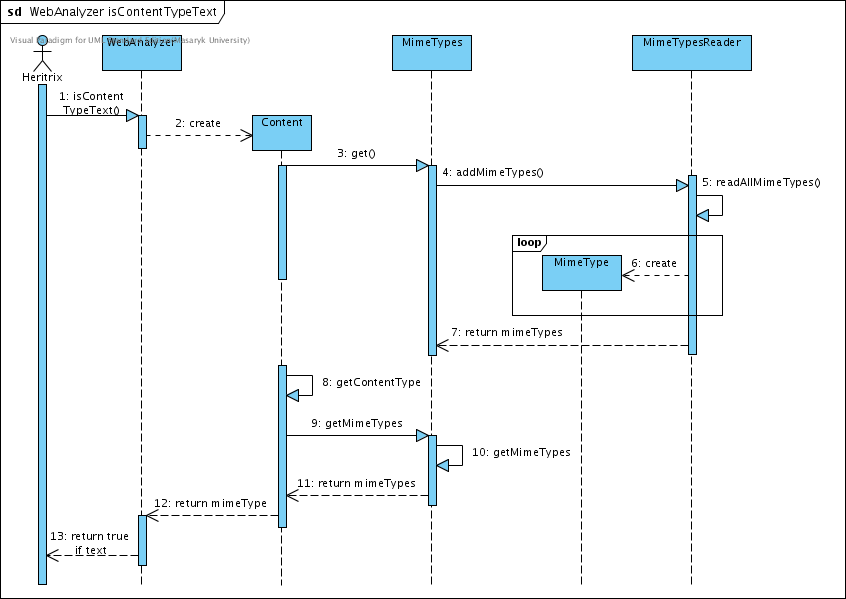
\includegraphics[width=120mm]{SD2.png}
\end{center}

Before analyzing the document it's important to identify its mime type. The text analyzing of binary document doesn't have sense. But user may want to identify the analyzed document only on the basis of URI name or IP address. Than the user has to deny all searchers that use text content to analyze the URI. Only searchers like GeoIPSearcher can be allowed in that case.

When the MimeTypeDetector is used for the first time, the Content object calls \emph{init()} method, that initializes all necessary objects. MimeTypesReader reads all elements from external xml document and creates MimeType instances from them. These instances are than stored into the collection of object MimeTypes. Now everything's prepared for identifing the unknown documents.

\subsection{The Analyzis}

\begin{center}
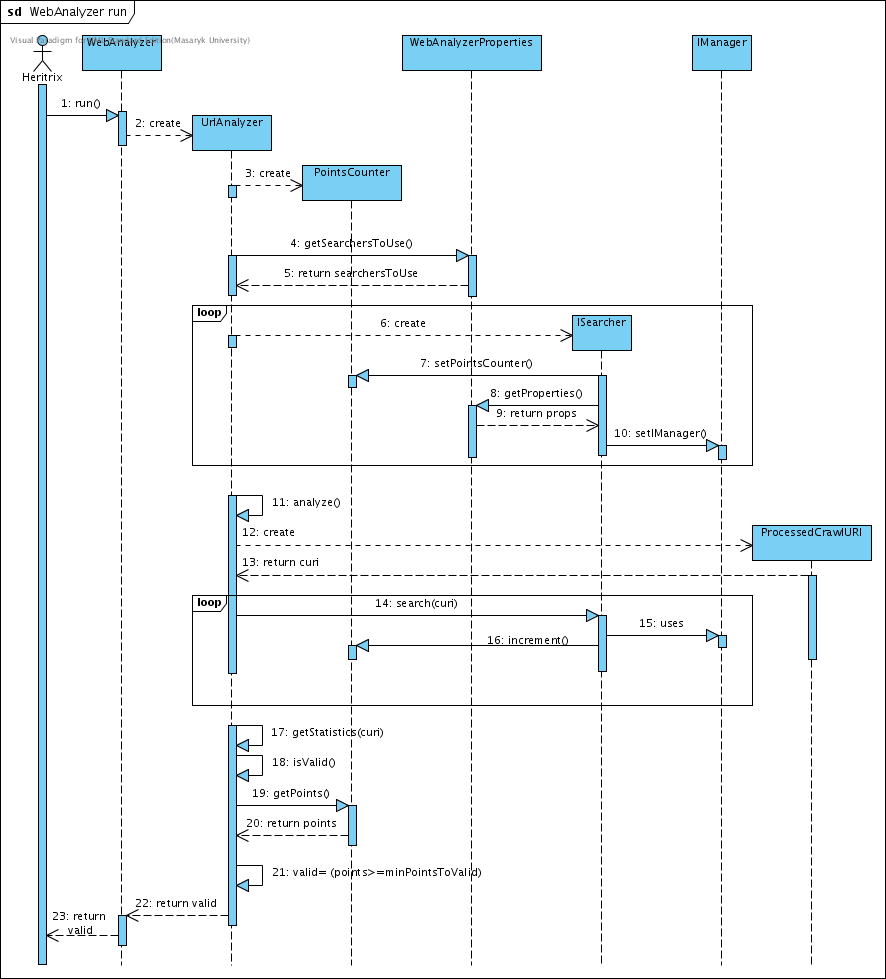
\includegraphics[width=120mm]{SD3.png}
\end{center}

The initialized WebAnalyzer is ready to analyze the URI. WebAnalyzer accepts some parametres of processed CrawlURI such as content, name and discovered links. Everytime when the Heriritrx calls WebAnalyzer to analyze the URI, new instance of UrlAnalyzer object is created. We prefer each thread has its own UrlAnalyzer instance, so that many threads can analyze the documents.

For each UrlAnalyzer new instance of PointsCounter is created and associated with it. According to the properties defined by the user all required searchers are instantiated. Each instance of ISearcher is associated with PointsCounter object, for searchers to be able to increment points of analyzed document, when relevant information is found. Some of the searches uses theirs managers. These managers provides synchronized methods, that accesses to files and databases. On the basis of reached points, the UrlAnalyzer decides whether the analyzed document is valid or not. Having received confirmation, that the processed URI is valid, Heritrix hanles it as we described above.

\subsection{The Finalization}

\begin{center}
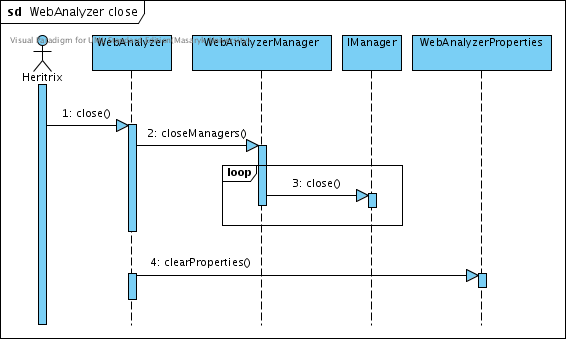
\includegraphics[width=120mm]{SD4.png}
\end{center}

When the whole process of crawl job is finished, it's necessaryto finalize the WebAnalyzer instance, so that it can be used in next crawl job. The WebAnalyzer instance is closed simultaneously with ExtractorWebAnalyzer processor. All managers in WebAnalyzer close opened database connections, files and streams.

\subsection{The Configuration}

Before we start the crawl job we have to configure both systems.

\subsubsection{Heritrix}
The configuration of Heritrix is easy. Just follow the steps in Heritrix user manual. If you want to use WebAnalyzer, you have to add ExtractorWebA\-na\-ly\-zer to extractors, replace ARCWriterProcessor by ARCWriterProcessorWebAnalyzer and replace original LinksScoper by LinksScoperWebAnalyzer. These three processor are required by WebAnalyzer. If you want to crawl the web outside the national domain you have to add some DecidingRules to filter out links from national domain (\emph{MatchesRegExpDecideRule}). We use the following DecidingRules in given order: \emph{AcceptDecideRule, Pa\-tho\-lo\-gi\-calPathDecideRule, TooManyPathSegmentsDecideRule, MatchesRegExpDecideRule}. Some further information is available in user manual.

\subsubsection{WebAnalyzer}
The configuration of WebAnalyzer works on the basis of configuration file \emph{webanalyzer.properties}. In this file you can find properties and their values used by WebAnalyzer.

\begin{description}
\item[webanalyzer.urlanalyzer.min.valid.points=200] - This property defines how many points must analyzed document reach to be identified as valid.
\item[webanalyzer.urlanalyzer.depth.toarchive=3] - This property is used by Heritrix to archive links referenced from valid URI. If value equals 0, than only valid URI with its sources (images, css styles,...) is archived. If we set the value to 3, it means that all links referenced from valid URI will be archived automatically to this level.
\end{description} 

other properties are used by concrete searchers:
\begin{description}
\item[properties for EmailSearcher]
\item[webanalyzer.searcher.email.use=1] - This means that the user wants to use EmailSearcher to analyze the document. Value 0 disables this searcher.
\item[webanalyzer.searcher.email.regexp=][a-z0-9.\_-]+@[a-z0-9.\_-]+$\backslash$$\backslash$.cz] - EmailSearcher searches all e-mails in the document. On the basis of this regular expression the user is able to define which e-mails are in his interest. This regular expression searches e-mails with .cz domain.
\item[webanalyzer.searcher.email.point=1] - When the relevant e-mail is found this value is added to reached points of analyzed URI.
\end{description}

Other properties of searchers are very similar.

\subsection{Components of WebAnalyzer}
WebAnalyzer analyzes the URI on the baseis of searchers, that are modular, so it's easy to add new module if you're skilled developer. All searchers perform very similar activities. They looks for relevant information in the ProcessedCrawlURI object. Some searchers work with text content of URI, others use its name or IP address. When the relevant information is found, searcher increments points of analyzed URI.

\subsubsection*{EmailSearcher}
Simple searcher based on the regular expression, that searches emails in text content of processed URI.

\subsubsection*{PhoneSearcher}
Simple searcher based on the regular expression, that searches phone numbers in text content of processed URI. The User is able to define in \emph{web\-a\-na\-lyzer.properties} file which phone numbers are in his interest. This searcher uses functionality of FilterText object to filter out source code from document  e.g. javascript.

\subsubsection*{HtmlLangSearcher}
Simple searcher based on the regular expression, that searches lang attributes in html source code of processed URI.

\subsubsection*{GeoIPSearcher}
The interesting criterion is code of country, from which the analyzed URI and URI's discovered links comes from. This searcher uses the project \emph{MaxMind}. The \emph{MaxMind} is able to find out the geological localization of concrete IP address. The version called \emph{GeoLiteCountry} is released for free and we can use it in our WebAnalyzer. This searcher uses its associated manager, that cooperates with \emph{GeoLiteCountry} interface. Some further information about MaxMind can be found on \url{http://www.maxmind.com}.

\subsubsection*{DictSearcher}
This component is able to search words in defined dictionary. It uses its own list of words with associated index for faster searching. If the word from text content of URI is found in this dictionary, searcher increments points of analyzed URI. The text content of URI is processed by FilterText object to filter out unrelevant block of text, such as source code. The DictSearcher uses its manager that cooperates with dictionary file and index file. The dictionary(wordlist) is created from czech corpus and contains no words occuring in other corpuses(slovak, english).

\subsubsection*{In Future we want to implement these Searchers}

\subsubsection*{TrigramSearcher}
TrigramSearcher will be able to identify the language of URI's text, on the basis of trigrams. This method seems to be quite precise, as we heard from the laboratory processing natural language.

\subsubsection*{URLSearcher}
The URLSearcher searches the URLs with specified domain in collection of discovered links.

\subsubsection*{ValidLinkSearcher}
This searchers checks whether the link discovered in analyzed URI is valid link. We gain the list of valid links from famous portals of concrete nation. In Czech republic it can be portal \emph{www.seznam.cz}. These links are considered to be important for the nation, and if analyzed URI contains some of these links, it means that it has something to do with the nation. This searcher uses \emph{Apache Lucene} project to index and search links.

\subsubsection*{ForbiddenLinkSearcher}
There are many links refering to sites with pornographic content. So it's a good thing to check whether the analyzed URI contains this sort of links. If forbidden link is found
we reduce points of analyzed URI. This will ensure that we won't archive pornographic webpages. The \emph{Apache Lucene} will be suitable for this job. 

\subsubsection*{ForbiddenDictSearcher}
ForbiddenDictSearcher will search vulgar words, because we don't want to archive vulgar webpages. The most important thing is to gain some list of vulgar words. The implementation will be very similar to DictSearcher.

\subsubsection*{CitySearcher}
The next module that can be usefull is CitySearcher. We just have to gain the list of cities of concrete nation. We can use \emph{Apache Lucene} project to implement this module.

\subsubsection*{GoogleSearcher}
In the future we want to implement searcher, that will use some functions from \emph{GoogleAPI}, but we don't have exact idea so far.

%================================NEW SECTION================================%

\newpage
\section{Testing}

The system hasn't run till the end so far. We was testing it only for 24 hours, due to lack of disk space. The system is still under construction and we expect that new errors may occur during the complete test, which may take few weeks.

Some statistics from test. The system analyzed 450 URIs in 2 minutes. The collection of seeds consisted of URIs outside the national domain.

\begin{center}
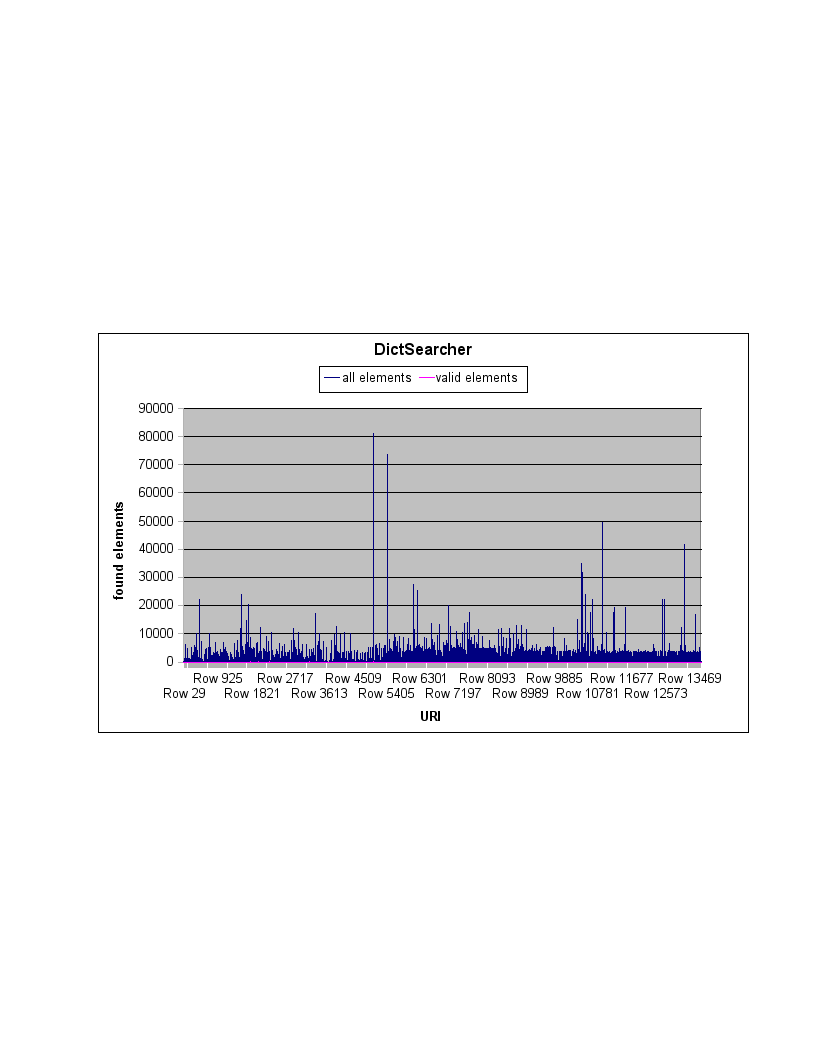
\includegraphics[width=135mm]{dict.png}


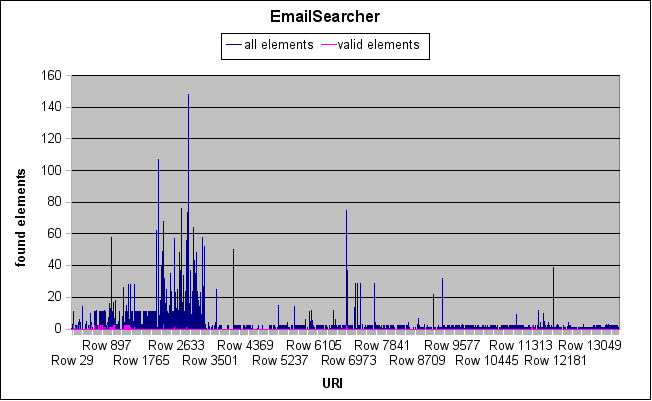
\includegraphics[width=135mm]{email.png}


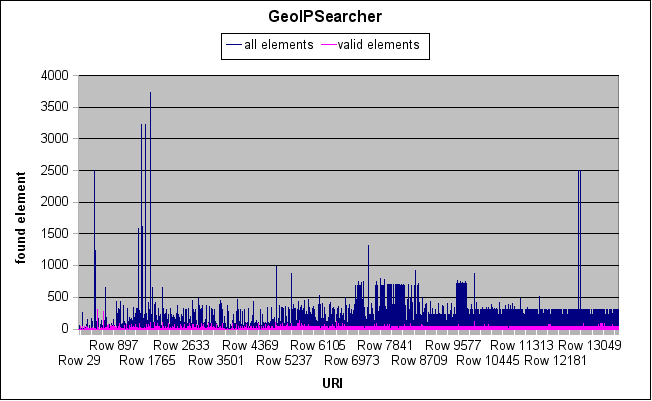
\includegraphics[width=135mm]{geo.png}


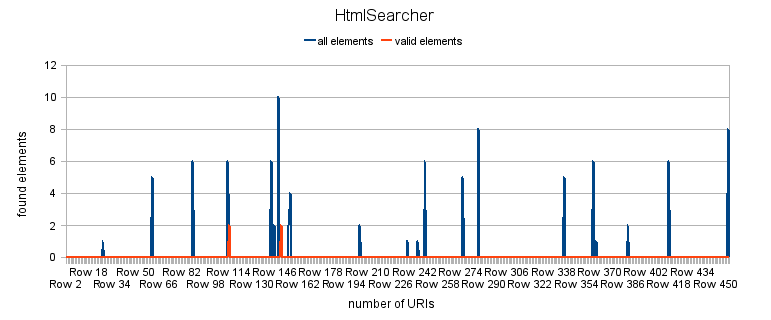
\includegraphics[width=135mm]{html.png}
\end{center}

%================================NEW SECTION================================%

\newpage
\section{The Conclusion}

We have to mention that the system si still under construction and we will develop new criteria to identify URIs. When we gain more experience with the system, we will upgrade it to meet new requirements that may occur during the running. We will try to develop the system to be modular, for us to add new functionality easily. 

In the future the system will be able to identify not only Czech web but also web of other nations. The only importatnt thing for identifing the web of other nations is to gain relevant sources that are used by WebAnalyzer (list of words, relevant URIs). Next importatnt milestone will be a new version of \emph{Heritrix 2}. We will try to adapt to this new version. It can be also a good oportunity to use new functionality that comes with \emph{Heritrix 2}. The WebAnalyzer is open-source system and we hope that some people will find it useful.

%================================NEW SECTION================================%

\newpage
\section{Sources}

\begin{itemize}
\item http://www.webarchiv.cz
\item http://crawler.archive.org/articles/developer\_manual/overview.html
\end{itemize}

\end{document}